%% This is file `example.tex',
%% generated with the docstrip utility.
%% The original source files were:
%% coppe.dtx  (with options: `example')
%% This is a sample monograph which illustrates the use of `coppe' document
%% class and `coppe-unsrt' BibTeX style.
%% \CheckSum{1311}
%% \CharacterTable
%%  {Upper-case    \A\B\C\D\E\F\G\H\I\J\K\L\M\N\O\P\Q\R\S\T\U\V\W\X\Y\Z
%%   Lower-case    \a\b\c\d\e\f\g\h\i\j\k\l\m\n\o\p\q\r\s\t\u\v\w\x\y\z
%%   Digits        \0\1\2\3\4\5\6\7\8\9
%%   Exclamation   \!     Double quote  \"     Hash (number) \#
%%   Dollar        \$     Percent       \%     Ampersand     \&
%%   Acute accent  \'     Left paren    \(     Right paren   \)
%%   Asterisk      \*     Plus          \+     Comma         \,
%%   Minus         \-     Point         \.     Solidus       \/
%%   Colon         \:     Semicolon     \;     Less than     \<
%%   Equals        \=     Greater than  \>     Question mark \?
%%   Commercial at \@     Left bracket  \[     Backslash     \\
%%   Right bracket \]     Circumflex    \^     Underscore    \_
%%   Grave accent  \`     Left brace    \{     Vertical bar  \|
%%   Right brace   \}     Tilde         \~}
%

%Escolher uma das 3 possibilidades no primeiro argumento
% msc - dissertacao de mestrado
% dscexam - qualificacao
% dsc - tese de doutorado
% tcc - trabalho de conclusão de curso
%
\documentclass[tcc,divps,pdftex]{tcc_modelo}
\usepackage[brazil]{babel}
\usepackage[utf8]{inputenc}
\usepackage{amsmath,amsthm,amsfonts,amssymb,enumerate}
\usepackage{setspace}
\usepackage[lined,boxed,portugues]{}
\usepackage{booktabs}
\usepackage[portuguese,algoruled,longend,linesnumbered]{algorithm2e}
\usepackage{natbib}
\usepackage{subfigure}
\usepackage{subeqnarray}
\usepackage{enumerate}
\usepackage{multicol}
%\usepackage{slashbox}

\usepackage{cases}
\usepackage{float}
\usepackage{soul}

\usepackage{pdfpages}

\usepackage{float}

\usepackage{listings}

\usepackage{xcolor,colortbl}         % Pacote de cores
\usepackage{bm}


\renewcommand{\lstlistingname}{Algoritmo}
\renewcommand{\algorithmcfname}{Pseudocódigo}


\newcommand{\R}{\mathbb{R}}
\newcommand{\N}{\mathbb{N}}
\newcommand{\Z}{\mathbb{Z}}
\newcommand{\Q}{\mathbb{Q}}
\newcommand{\K}{\mathbb{K}}
\newcommand{\I}{\mathbb{I}}
\newcommand{\id}{\mathbf{1}}
\newcommand{\U}{\mathcal{U}}
\newcommand{\V}{{\cal V}}

\newcommand{\mat}[1]{\mbox{\boldmath{$#1$}}}


\newtheorem{teo}{Teorema}[chapter]

%\hyphenation{ca-pi-tal}



\sloppy
\hyphenpenalty=10000

%\makelosymbols
%\makeloabbreviations
%\makenomenclature
% \makeglossary
%\usepackage{titlesec}
%\titleformat{\section}{\bfseries\normalsize}{\uppercase{\sectiontitle}\thesection.\quad}{1em}{}

\begin{document}

\course{ENGCOMP} %engenharia Computacional
\institute{FACENG_ICE} %Faculdade de Engenharia e Instituto de Ciências Exatas

\title{Heurísticas de Busca em Vizinhança para Roteamento por Segmentos Adaptativo no Tempo}%Possível título
%\foreigntitle{To be defined...}

\author{}{Pedro Henrique de Souza Rodrigues}

\advisor{Prof.}{Nome}{Orientador}{D.Sc.}{Universidade}
\coadvisor{}{}{}{}{}
\coadvisorII{}{}{}{}{}

\examinerI{Prof.}{Membro da Banca 1}{D.Sc.}{Universidade }
\examinerII{Prof.}{Membro da Banca 2}{D.Sc.}{Universidade }
\examinerIII{}{}{}{}
\examinerIV{}{}{}{}



%definir data da defesa
\date{20}{07}{2024}

%Palavras chaves do resumo em portugues
\keyword{Segment Routing}
\keyword{Engenharia de Tráfego}
\keyword{Meta-heurísticas}
\keyword{Busca em Vizinhança Variável}
\keyword{Desafio EURO/ROADEF 2026}

%Palavras chaves do abstract em ingles
\keywordEN{Segment Routing}
\keywordEN{Traffic Engineering}
\keywordEN{Metaheuristics}
\keywordEN{Variable Neighborhood Search}
\keywordEN{EURO/ROADEF 2026 Challenge}


\inserecapa

\maketitle

\frontmatter

\dedication{A quem você dedica o trabalho...}

 \begin{agradecimentos}

Agradeço ...
 \end{agradecimentos}
 
 \epigrafe{``Frase que te inspirou''  \flushright{(Autor)}}

\begin{abstract}
Este trabalho trata o problema de \textit{Segment Routing} adaptativo no tempo (T-ASR), proposto no desafio EURO/ROADEF 2026: escolher, para cada demanda de uma rede IP e em cada período, uma lista de nós intermediários que minimize a carga dos enlaces mais carregados, considerando intervenções de manutenção e um orçamento que limita as reconfigurações entre períodos. São propostas duas meta-heurísticas de busca em vizinhança, uma busca adaptativa em múltiplas vizinhanças (AMNS) e uma descida em vizinhança variável com perturbação (VND), que compartilham uma avaliação de cargas idêntica à do avaliador oficial, incluindo a divisão de tráfego por múltiplos caminhos de mesmo custo, e uma fase robusta que planeja o primeiro período considerando as intervenções de todo o horizonte. Nas 56 instâncias públicas dos conjuntos A, B, C e X, os métodos reduziram a utilização máxima do pior período em cerca de 46\% em média em relação ao roteamento sem otimização, com soluções válidas segundo o avaliador oficial, e eliminaram todas as violações de capacidade nos conjuntos A, B e X.
\end{abstract}

\begin{foreignabstract}
This work addresses the T-Adaptive Segment Routing problem (T-ASR) of the EURO/ROADEF 2026 challenge: for each demand of an IP network and each time period, choose a list of intermediate nodes that minimizes the load of the most loaded links, under maintenance interventions and a budget that limits reconfigurations between periods. Two neighborhood search metaheuristics are proposed, an Adaptive Multi-Neighborhood Search (AMNS) and a Variable Neighborhood Descent with shaking (VND). They share a load evaluation identical to the official checker, including Equal-Cost Multi-Path traffic splitting, and a robust phase that plans the first period against the interventions of the whole horizon. On the 56 public instances of sets A, B, C and X, the methods reduced the worst-period maximum link utilization by about 46\% on average compared with non-optimized routing, with all solutions accepted by the official checker, and removed every capacity violation in sets A, B and X.
\end{foreignabstract}



% \clearpage


\listoffigures  %Com titulo : lista de ilustracoes
\listoftables

%----Glossário ------------
\clearpage
\clearpage
\begin{center}
\textbf{LISTA DE ABREVIAÇÕES E SIGLAS}
\end{center}

\vspace*{1.cm}

\doublespacing  \begin{tabular}{l l}
ALNS&    \textit{Adaptive Large Neighborhood Search}\\
AMNS&    \textit{Adaptive Multi-Neighborhood Search}\\
ECMP&    \textit{Equal-Cost Multi-Path}\\
IETF&    \textit{Internet Engineering Task Force}\\
IGP&     \textit{Interior Gateway Protocol}\\
IP&      \textit{Internet Protocol}\\
MLU&     \textit{Maximum Link Utilization}\\
MPLS&    \textit{Multiprotocol Label Switching}\\
SR&      \textit{Segment Routing}\\
TE&      \textit{Traffic Engineering}\\
T-ASR&   \textit{T-Adaptive Segment Routing}\\
VND&     \textit{Variable Neighborhood Descent}\\
VNS&     \textit{Variable Neighborhood Search}\\
\end{tabular}  \thispagestyle{empty}
 %arquivo abreviacoes.tex não é automatizado :/

\tableofcontents


\mainmatter

%------------------------------------------------------------------------------

%deixei uma introdução para tomar como exemplo, algumas formataçoes não foram automaticas e são feitas manualmente no .tex
% capitulos/introducao.tex: rascunho original, incorporado ao capitulo 3
% \chapter{INTRODUÇÃO}


\section{\uppercase{Motivação e Contextualização}}

\section{TRABALHOS RELACIONADOS}

\chapter{DESCRIÇÃO DO PROBLEMA}

O problema a ser tratado consiste em determinar um esquema de roteamento para uma rede e que seja, simultaneamente, eficiente e resiliente a falhas de equipamentos ou enlaces. A natureza do esquema de roteamento não é estático: ele deve ser capaz de se adaptar a diferentes cenários ao longo do tempo, especialmente durante intervenções de manutenção programadas e na ocorrência de falhas não planejadas.

Formalmente, o problema recebe como entrada:

1.  Topologia da Rede: Um grafo que representa os roteadores (nós) e os enlaces de comunicação (arestas) da rede, também chamados de links. Cada link possui 2 atributos: uma métrica, que equivale a distância física entre os nós, e uma capacidade, que limita o máximo de fluxo que o link consegue suportar
    (IMAGEM)

2.  Matriz de Tráfego: A demanda de tráfego entre os pares origem-destino que deve ser roteada.

    (IMAGEM)
    
3.  Janelas de Manutenção: Períodos programados durante os quais determinados links ficam indisponíveis para manutenção.

    (IMAGEM)
    
4.  Orçamento de Reconfiguração: Um limite para a frequência e extensão das mudanças no esquema de roteamento, imposto para controlar os custos operacionais e o risco de instabilidade na rede.

    (IMAGEM)

O objetivo principal é computar um esquema de roteamento baseado em Segment Routing (SR) que minimize o fluxo de demandas nos links mais carregados e garantindo que essa carga permaneça dentro de limites aceitáveis mesmo quando a rede sofre uma falha (seja um enlace ou um nó). O esquema deve ser adaptativo o suficiente para lidar com as janelas de manutenção e, ao mesmo tempo, respeitar o orçamento de reconfiguração disponível.

\section{MODELO MÁTEMATICO}


Para modelar corretamente o problema, será necessário considerar um conjunto de restrições que podem ser agrupadas nas seguintes categorias:

#### 1. Restrições de Roteamento e Capacidade

As restrições fundamentais de um problema de reteamento de dados:

- Conservação de Fluxo: Para cada par origem-destino, o fluxo de tráfego deve ser integralmente roteado da origem ao destino. Não pode haver perda de tráfego.
- Capacidade máxima dos links: A soma de todo o tráfego roteado através de um enlace não pode exceder sua capacidade nominal.

2. Restrições de Falhas

- Cenários de Falha: Durante uma janela de manutenção, certos links são explicitamente removidos da topologia. O esquema de roteamento deve ser capaz de operar corretamente (isto é, rotear todo o tráfego) mesmo com esses recursos ausentes.

3. Restrições de Orçamento de Reconfiguração

Esta é uma restrição que diferencia o desafio de problemas de roteamento estático tradicionais:

- Limite de Mudanças: O número de vezes que o esquema de roteamento pode ser alterado (por exemplo, ao longo de um horizonte de tempo ou entre diferentes cenários) é limitado por um orçamento. Cada mudança no esquema de SR tem um custo associado.

4. Restrições Específicas do Segment Routing

- Profundidade Máxima de Segmentos: O número de segmentos (rótulos) que um pacote pode carregar é limitado na intância do problema A solução deve respeitar esse limite.

\chapter{INTRODUÇÃO}
\label{cap:introducao}

\section{\uppercase{Motivação e Contextualização}}

Operadoras de telecomunicações mantêm grandes redes IP/MPLS (\textit{Internet Protocol / Multiprotocol Label Switching}) com milhares de roteadores e enlaces, por onde trafegam dezenas de milhares de demandas entre pares origem-destino. Nessas redes, os pacotes são tradicionalmente encaminhados pelos caminhos mínimos calculados por um protocolo de roteamento interno (IGP, \textit{Interior Gateway Protocol}) a partir de pesos atribuídos aos enlaces. Esse esquema é simples de operar, mas dá pouco controle sobre a distribuição da carga: enlaces que pertencem a muitos caminhos mínimos ficam sobrecarregados enquanto outros permanecem ociosos.

A Engenharia de Tráfego (TE, \textit{Traffic Engineering}) busca usar melhor a infraestrutura existente, evitando congestionamentos e garantindo qualidade de serviço. Uma métrica central é a utilização máxima dos enlaces (MLU, \textit{Maximum Link Utilization}), isto é, a carga do enlace mais carregado da rede. Reduzir a MLU dá margem para absorver picos de tráfego e falhas.

O \textit{Segment Routing} (SR) é uma tecnologia que permite desviar o tráfego dos caminhos mínimos sem alterar os pesos do IGP: cada pacote carrega uma lista de nós intermediários (\textit{waypoints}) que deve visitar em ordem, e entre dois \textit{waypoints} consecutivos o encaminhamento continua sendo feito pelos caminhos mínimos. Com poucos \textit{waypoints} por demanda é possível redistribuir a carga de forma eficaz.

O desafio EURO/ROADEF 2026, proposto pela Orange, acrescenta uma dimensão temporal a esse problema. O horizonte é dividido em períodos (\textit{time slots}); em cada período, o volume das demandas muda e alguns enlaces ficam indisponíveis por intervenções de manutenção. O esquema de SR pode ser reconfigurado de um período para o seguinte, mas cada mudança tem custo operacional, e o número de segmentos alterados entre períodos consecutivos é limitado por um orçamento. O problema resultante, chamado \textit{T-Adaptive Segment Routing} (T-ASR), combina a escolha de rotas, a resiliência a indisponibilidades e o controle das reconfigurações.

\section{\uppercase{Objetivos}}

O objetivo geral deste trabalho é desenvolver e avaliar heurísticas de busca em vizinhança para o problema T-ASR do desafio EURO/ROADEF 2026, capazes de produzir esquemas de \textit{Segment Routing} válidos e com baixa utilização máxima dos enlaces em todos os períodos.

Os objetivos específicos são:
\begin{itemize}
    \item modelar o cálculo de cargas exatamente como o avaliador oficial do desafio, incluindo a divisão de tráfego por múltiplos caminhos de mesmo custo (ECMP, \textit{Equal-Cost Multi-Path});
    \item implementar duas meta-heurísticas sobre as mesmas vizinhanças: uma busca adaptativa em múltiplas vizinhanças (AMNS, \textit{Adaptive Multi-Neighborhood Search}) e uma Descida em Vizinhança Variável (VND, \textit{Variable Neighborhood Descent}) combinada com perturbações (VNS);
    \item tratar a dependência entre períodos causada pelo orçamento de reconfiguração, planejando o primeiro período em função de todos os períodos seguintes;
    \item comparar os métodos entre si e com uma solução trivial sem otimização, usando as instâncias públicas do desafio e o avaliador oficial.
\end{itemize}

\section{\uppercase{Organização do Trabalho}}

O Capítulo~\ref{cap:fundamentacao} apresenta os conceitos de roteamento IGP, ECMP, \textit{Segment Routing}, engenharia de tráfego e as meta-heurísticas usadas, além de trabalhos relacionados. O Capítulo~\ref{cap:problema} descreve o problema T-ASR e seu modelo matemático. O Capítulo~\ref{cap:metodologia} detalha os métodos propostos e sua implementação. O Capítulo~\ref{cap:resultados} apresenta os experimentos computacionais e discute os resultados. Por fim, o Capítulo~\ref{cap:conclusao} traz as conclusões e os trabalhos futuros.

\chapter{FUNDAMENTAÇÃO TEÓRICA}
\label{cap:fundamentacao}

\section{\uppercase{Roteamento por Caminhos Mínimos e ECMP}}

Em uma rede IP, cada enlace recebe um peso (métrica) e os roteadores calculam, com o algoritmo de Dijkstra, os caminhos de menor peso total até cada destino. Quando existem vários caminhos mínimos entre dois nós, o mecanismo ECMP (\textit{Equal-Cost Multi-Path}) divide o tráfego entre eles.

Seja $G = (V, A)$ a rede, com métrica $\omega(a)$ em cada arco. O grafo de encaminhamento $FG(u, v)$ é o subgrafo formado por todos os arcos que pertencem a algum caminho mínimo de $u$ até $v$. Pela regra ECMP, o fluxo que chega a um nó de $FG(u, v)$ é dividido igualmente entre os arcos de saída desse nó em $FG(u, v)$. A fração do fluxo de $u$ para $v$ que passa pelo arco $a$ é o coeficiente de divisão $r(u, v, a)$, nulo se $a \notin FG(u, v)$.

\section{\uppercase{Segment Routing}}

O \textit{Segment Routing} (SR) permite que a origem defina uma sequência de nós que o pacote deve visitar, codificada no próprio cabeçalho. Um caminho de segmentos para uma demanda de $s$ para $t$ é uma sequência $\langle s, w_1, \dots, w_\ell, t \rangle$, em que $w_1, \dots, w_\ell$ são os \textit{waypoints}. Cada par consecutivo é um segmento, e entre os extremos de um segmento o tráfego segue o grafo de encaminhamento $FG$ do IGP. Sem \textit{waypoints} ($\ell = 0$), a demanda é roteada pelos caminhos mínimos de $s$ a $t$.

A vantagem do SR para a engenharia de tráfego é que poucos segmentos bastam para desviar demandas de enlaces congestionados, sem alterar a métrica de nenhum enlace e, portanto, sem afetar o restante do tráfego.

\section{\uppercase{Engenharia de Tráfego e Utilização dos Enlaces}}

A carga (utilização) de um enlace é a razão entre o fluxo que passa por ele e sua capacidade; valores acima de 1 indicam congestionamento. A utilização máxima dos enlaces (MLU) é o critério mais usado em engenharia de tráfego. Abordagens clássicas otimizam os pesos do IGP; com SR, a otimização passa a ser a escolha dos \textit{waypoints} de cada demanda. O desafio EURO/ROADEF 2026 estende o critério para uma ordem lexicográfica: minimiza-se o enlace mais carregado, depois o segundo mais carregado, e assim por diante, considerando todos os períodos.

\section{\uppercase{Meta-heurísticas de Busca em Vizinhança}}

Uma busca local parte de uma solução e a substitui repetidamente por uma solução vizinha melhor, até atingir um ótimo local. A vizinhança é definida por um tipo de movimento, como inserir ou trocar um \textit{waypoint}.

A \textbf{Descida em Vizinhança Variável} (VND) explora várias vizinhanças em ordem fixa: ao encontrar uma melhora, volta para a primeira; ao esgotar todas, termina em uma solução que é ótimo local para todas elas. A \textbf{Busca em Vizinhança Variável} (VNS) combina essa descida com perturbações (\textit{shaking}) que tiram a busca do ótimo local, aceitando a nova solução apenas se ela for melhor que a melhor conhecida.

Buscas adaptativas, como a ALNS (\textit{Adaptive Large Neighborhood Search}), sorteiam a vizinhança a aplicar em cada iteração, com pesos que aumentam para os movimentos que mais trouxeram melhorias. A AMNS usada neste trabalho segue essa ideia: os pesos dos movimentos se adaptam ao longo da busca, e a VNS é usada para escapar de ótimos locais.

\section{\uppercase{Trabalhos Relacionados}}

Fortz e Thorup (2000) mostraram que otimizar os pesos do OSPF reduz significativamente o congestionamento, mas qualquer mudança de peso afeta todo o tráfego que usa o enlace. Bhatia et al. (2015) formularam a engenharia de tráfego com \textit{Segment Routing} e mostraram que poucos segmentos por demanda já aproximam o roteamento ótimo. O desafio EURO/ROADEF 2026 introduz a versão temporal com intervenções e orçamento de reconfiguração; as soluções publicadas na fase \textit{sprint} do desafio são uma referência de comparação natural.

\citet{yang2023intelligent} tratam o balanceamento de carga com SR sob um limite para o tamanho do cabeçalho de segmentos, que representa o custo de controle do SR. No esquema proposto, o IRTE, um controlador centralizado coleta o estado da rede e decide, para cada fluxo, se ele segue o caminho mínimo ou um caminho de desvio que passa por nós de desvio escolhidos, com um limite para o número de rótulos de desvio por fluxo. Os autores formulam a escolha como um problema de mapeamento de fluxos a nós de desvio, mostram que ele é NP-difícil por redução ao problema do subgrafo $k$-denso e propõem dois algoritmos: o LBA-DR, baseado em programação linear com arredondamento aleatório, e o IACO, uma otimização por colônia de formigas. Em seis topologias reais do \textit{Internet Topology Zoo}, com 11 a 125 nós, a utilização máxima de banda foi até 24,6\% menor que a do roteamento tradicional, na topologia BellCanada. O objetivo (a carga do enlace mais carregado) e o limite de segmentos por caminho são os mesmos do problema tratado neste trabalho; o problema deles, porém, considera uma única configuração da rede, sem falhas nem custo de reconfiguração ao longo do tempo, e as redes avaliadas são bem menores que as do desafio, que chegam a 3902 nós.

\citet{aubry2018robustly} exploram uma propriedade do SR que também é central neste trabalho: quando um enlace falha, o IGP recalcula os caminhos mínimos e a mesma lista de segmentos passa a corresponder a outro caminho, sem nenhuma reconfiguração. Os autores definem pares de caminhos robustamente disjuntos, que permanecem disjuntos para qualquer falha de um conjunto dado pelo operador, e buscam o par com o menor atraso no pior caminho. Eles provam que o problema é NP-difícil em geral, mas que se torna tratável em tempo polinomial quando o número máximo de segmentos por caminho é fixo, e usam uma condição necessária e suficiente para a robustez para podar o espaço de busca. Em topologias do Rocketfuel e do \textit{Internet Topology Zoo}, os caminhos são calculados em frações de segundo ou poucos segundos na maioria dos casos, e um único nó intermediário eleva a fração de pares origem-destino com caminhos robustamente disjuntos para 71\% a 100\%, enquanto desvios adicionais trazem pouco ganho. A fase robusta deste trabalho segue a mesma ideia, com outro objetivo: escolher, no primeiro período, listas de segmentos cujos caminhos continuem bons depois das intervenções dos períodos seguintes, recalculados pelo IGP. A pouca utilidade de desvios adicionais também tem um análogo aqui, com o teste da inserção dupla de \textit{waypoints} (Seção~\ref{sec:insercao_dupla}).

\citet{chen2022waypoint} aplicam SR a redes de satélites de órbita baixa (LEO), cuja topologia muda com o movimento dos satélites. O tempo é dividido em intervalos de topologia fixa, e os enlaces entre planos orbitais são desligados quando os satélites entram nas regiões polares. Como essas mudanças são previsíveis, os autores escolhem até dois \textit{waypoints} por caminho para que a rota evite, já no intervalo atual, os enlaces que serão desligados no intervalo seguinte. O problema é formulado como programação não linear inteira mista e resolvido em etapas: os enlaces que serão desligados são removidos do grafo, o caminho mínimo é calculado com o algoritmo de Dijkstra, e os \textit{waypoints} são escolhidos entre os nós da mesma órbita da origem e do destino. Em simulações com o NS-3, o algoritmo teve menos perda de pacotes, atraso e variação de atraso que o OLSR. Assim como no desafio, as indisponibilidades de enlaces são conhecidas com antecedência e as rotas são escolhidas para atravessá-las sem reconfiguração; o objetivo, porém, é a estabilidade e o número de saltos de cada caminho, e não a carga dos enlaces, e não há orçamento de reconfiguração.

Em resumo, os trabalhos revisados tratam separadamente aspectos que o problema T-ASR combina: o balanceamento de carga com poucos segmentos por caminho \citep{yang2023intelligent}, a robustez de listas de segmentos a falhas sem reconfiguração \citep{aubry2018robustly} e o planejamento de rotas para mudanças previsíveis na topologia \citep{chen2022waypoint}. Nenhum deles considera, ao mesmo tempo, a minimização da carga máxima em vários períodos com intervenções programadas e um orçamento que limita as mudanças de segmentos entre períodos, que é a combinação abordada neste trabalho.

\chapter{DESCRIÇÃO DO PROBLEMA}
\label{cap:problema}

O problema tratado consiste em determinar um esquema de roteamento para uma rede que seja, simultaneamente, eficiente e resiliente à indisponibilidade de enlaces. O esquema não é estático: ele deve se adaptar a diferentes cenários ao longo do tempo, em especial durante intervenções de manutenção programadas.

O problema recebe como entrada:

\begin{enumerate}
    \item \textbf{Topologia da rede}: um grafo direcionado que representa os roteadores (nós) e os enlaces de comunicação (arcos), também chamados de \textit{links}. Cada enlace possui dois atributos: uma métrica, usada pelo IGP para calcular os caminhos mínimos, e uma capacidade, que é a referência para a carga do enlace.
    \item \textbf{Matriz de tráfego}: o volume de tráfego de cada par origem-destino (demanda) em cada período.
    \item \textbf{Janelas de manutenção}: para cada período, o conjunto de enlaces indisponíveis por intervenções.
    \item \textbf{Orçamento de reconfiguração}: para cada período, um limite para o número de segmentos alterados em relação ao período anterior, imposto para controlar o custo operacional e o risco de instabilidade.
    \item \textbf{Profundidade máxima}: o número máximo de segmentos de um caminho de SR.
\end{enumerate}

\textbf{[INSERIR FIGURAS: exemplo de topologia, matriz de tráfego, intervenção e orçamento.]}

O objetivo é calcular, para cada período, um esquema de roteamento baseado em \textit{Segment Routing} que minimize a carga dos enlaces mais carregados, respeitando as intervenções, o orçamento de reconfiguração e a profundidade máxima.

\section{\uppercase{Modelo Matemático}}

A formulação a seguir segue a especificação oficial do desafio. Seja $G = (V, A, \omega, c)$ a rede, com métrica $\omega(a)$ e capacidade $c(a)$ em cada arco $a \in A$; $T$ o conjunto de períodos; $D$ o conjunto de demandas $d = (s_d, t_d)$ com volume $\lambda(d, t)$ no período $t$; $A_t \subseteq A$ os arcos disponíveis no período $t$ (sem os enlaces em intervenção); $\mathit{maxSeg}$ a profundidade máxima; e $\beta(t)$ o orçamento do período $t \geq 1$.

\paragraph{Variáveis.} $x^d_{ijt} \in \{0, 1\}$ vale 1 se o caminho de segmentos da demanda $d$ contém o segmento $(i, j)$ no período $t$.

\paragraph{Carga.} Com $r_t(i, j, a)$ o coeficiente de divisão ECMP do segmento $(i, j)$ no arco $a$, calculado no grafo $G_t = (V, A_t)$, a carga do arco $a$ no período $t$ é
\begin{equation}
    \ell(a, t) = \frac{1}{c(a)} \sum_{d \in D} \sum_{i, j \in V} r_t(i, j, a)\, \lambda(d, t)\, x^d_{ijt}.
\end{equation}

\paragraph{Restrições.}
\begin{itemize}
    \item \textbf{Conservação de fluxo}: para cada demanda e período, os segmentos escolhidos formam um caminho de $s_d$ até $t_d$:
    \begin{equation}
        \sum_{j \in V} x^d_{ijt} - \sum_{j \in V} x^d_{jit} =
        \begin{cases} 1 & \text{se } i = s_d,\\ -1 & \text{se } i = t_d,\\ 0 & \text{caso contrário,} \end{cases}
        \qquad \forall d \in D,\ i \in V,\ t \in T.
    \end{equation}
    \item \textbf{Profundidade máxima}: $\sum_{i, j \in V} x^d_{ijt} \leq \mathit{maxSeg}$, para todo $d \in D$ e $t \in T$.
    \item \textbf{Orçamento de reconfiguração}: o número de segmentos que entram ou saem dos caminhos entre períodos consecutivos é limitado:
    \begin{equation}
        \sum_{d \in D} \sum_{i, j \in V,\, i \neq j} \left| x^d_{ijt} - x^d_{ij,t-1} \right| \leq \beta(t), \qquad \forall t \geq 1.
    \end{equation}
    \item \textbf{Intervenções}: nos períodos em que um enlace está em intervenção, ele não existe em $G_t$, e o tráfego é encaminhado pelos caminhos mínimos que restam.
\end{itemize}

Diferentemente de formulações clássicas, a capacidade não é uma restrição rígida: cargas acima de 1 são permitidas, mas indicam congestionamento e pioram o objetivo.

\paragraph{Objetivo.} Minimizar, em ordem lexicográfica decrescente, o vetor das cargas $\ell(a, t)$ de todos os arcos em todos os períodos: primeiro a maior carga (a MLU de todo o horizonte), depois a segunda maior, e assim por diante.

\section{\uppercase{Instâncias}}

O desafio disponibiliza conjuntos de instâncias com dificuldade crescente. A Tabela~\ref{tab:instancias} resume os conjuntos usados neste trabalho. O conjunto C, da fase de qualificação, é o maior: até 3902 nós e 24 períodos.

\begin{table}[H]
\centering
\caption{Conjuntos de instâncias usados nos experimentos.}
\label{tab:instancias}
\begin{tabular}{lrrrrrr}
\toprule
Conjunto & Instâncias & Nós & Arcos & Demandas & Períodos & $\mathit{maxSeg}$ \\
\midrule
A & 20 & 20--400 & 80--2000 & 20--6000 & 2 & 6 \\
B & 12 & 264--1263 & 864--5036 & 2546--15000 & 12 & 8 \\
X & 12 & 264--1263 & 864--5036 & 2546--15000 & 12 & 8 \\
\bottomrule
\end{tabular}
\end{table}

Os orçamentos são pequenos em relação ao número de demandas: nos conjuntos B e X são de 10 a 78 segmentos por período para milhares de demandas, e no conjunto C variam de 0 a 30. Inserir um único \textit{waypoint} em uma rota custa 3 unidades de orçamento (remove um segmento e acrescenta dois). Consequentemente, o roteamento escolhido no primeiro período tende a valer, quase sem alterações, para todo o horizonte. Essa observação orienta o método proposto no Capítulo~\ref{cap:metodologia}.

\chapter{METODOLOGIA}
\label{cap:metodologia}

Este capítulo descreve os métodos propostos. As duas meta-heurísticas, AMNS e VND, compartilham a representação da solução, a avaliação das cargas, a função objetivo, as vizinhanças e uma fase robusta aplicada ao primeiro período; elas diferem apenas na forma de escolher e encadear os movimentos.

\section{\uppercase{Visão Geral}}

Os períodos são resolvidos em ordem. Em cada período $t$:
\begin{enumerate}
    \item calculam-se as distâncias mínimas entre todos os pares de nós no grafo $G_t$, sem os enlaces em intervenção;
    \item os \textit{waypoints} de cada demanda são inicializados com os do período anterior (no período 0, todas as rotas começam sem \textit{waypoints});
    \item a meta-heurística (AMNS ou VND) melhora a solução, respeitando o orçamento $\beta(t)$;
    \item no período 0, uma fase robusta reavalia as rotas considerando todos os períodos seguintes (Seção~\ref{sec:robusta});
    \item as rotas e cargas do período são registradas e os \textit{waypoints} seguem para o próximo período.
\end{enumerate}

\section{\uppercase{Representação e Avaliação}}

Uma solução associa a cada demanda e período uma lista de \textit{waypoints}. Para avaliá-la, cada segmento $(u, v)$ é convertido em frações de fluxo por arco, exatamente como faz o avaliador oficial: calcula-se o grafo de encaminhamento $FG(u, v)$ a partir das distâncias até $v$, e o fluxo que chega a cada nó é dividido igualmente entre seus arcos de saída em $FG(u, v)$, processando os nós em ordem decrescente de distância até $v$. As frações de cada segmento são guardadas em cache, pois os mesmos segmentos se repetem em muitas demandas e movimentos.

As distâncias são obtidas pelo algoritmo de Dijkstra a partir de cada nó. Como as métricas são inteiras, as somas são exatas, e os empates que ativam o ECMP são detectados sem erro numérico. Nos testes, as cargas calculadas coincidiram com as do avaliador oficial em todas as casas decimais.

Uma demanda $d$ contribui com $\lambda(d, t)\, r_t(i, j, a)$ ao fluxo de cada arco $a$ de cada segmento $(i, j)$. O fluxo agregado por arco é mantido de forma incremental: um movimento remove a contribuição antiga da demanda e acrescenta a nova.

\section{\uppercase{Função Objetivo}}

Em vez do vetor lexicográfico completo, que é caro de comparar, a busca usa uma aproximação lexicográfica com seis componentes, em ordem de prioridade:
\begin{enumerate}
    \item número de demandas sem rota;
    \item excesso total de carga, $\sum_a \max(0, \ell(a) - 1)$;
    \item carga máxima (MLU do período);
    \item número de enlaces na faixa próxima ao máximo (carga $\geq$ MLU $- 0{,}2\%$);
    \item no período 0, excesso quadrático dos enlaces ``quentes'', $\sum_a \max(0, \ell(a) - \tau)^2$, com $\tau$ igual à metade da MLU;
    \item soma dos quadrados das cargas, como desempate final.
\end{enumerate}
O quarto componente permite progredir em platôs: quando vários enlaces empatam no máximo, aliviar um deles já é uma melhora, antes que a MLU diminua. O quinto incentiva espalhar a carga sem penalizar rotas mais longas por enlaces vazios.

Enlaces cujo tráfego não pode ser evitado por nenhuma escolha de \textit{waypoints} (por exemplo, o único enlace de saída da origem de uma demanda) são ignorados na carga usada pela busca, pois fixariam o máximo e paralisariam a otimização do restante da rede. As cargas reportadas e avaliadas pelo avaliador oficial incluem esses enlaces normalmente.

\section{\uppercase{Vizinhanças}}

Todas as vizinhanças atuam sobre o \textbf{corte crítico}: os enlaces na faixa próxima ao máximo e as demandas que passam por eles, processadas em ordem decrescente de volume. Para cada demanda, sua contribuição é retirada da rede, e os nós candidatos a \textit{waypoint} são ordenados pela carga residual dos caminhos que criariam. Essa ordenação é feita com uma programação dinâmica sobre os grafos de caminhos mínimos (a partir da origem do segmento e até o seu destino), que dá, para todos os nós candidatos de uma vez, a maior carga nos grafos de encaminhamento resultantes. Os 16 melhores candidatos (32 no período 0) têm o objetivo calculado exatamente por avaliação incremental, e apenas os 3 melhores (5 no período 0) são de fato aplicados e testados.

\begin{itemize}
    \item \textbf{Inserção (\textit{insert})}: insere um \textit{waypoint} em um segmento da rota que cruza o corte crítico. É o principal ataque ao gargalo.
    \item \textbf{Troca (\textit{change})}: substitui um \textit{waypoint} cujos segmentos tocam o corte crítico. Diversifica quando a inserção estagna.
    \item \textbf{Remoção (\textit{delete})}: remove um \textit{waypoint} quando o atalho resultante não é mais carregado que o desvio atual. Simplifica rotas e recupera orçamento.
    \item \textbf{Extensão (\textit{extend})}: apenas no período 0, onde não há orçamento. Para demandas que passam por enlaces quentes, insere mais um \textit{waypoint} se isso mantém a MLU e reduz o excesso quadrático, levando tráfego para a parte fria da rede.
    \item \textbf{Perturbação (\textit{shake})}: aplica movimentos aleatórios entre os melhores candidatos, aceitando piora de até 2\% na MLU, para escapar de ótimos locais.
\end{itemize}

Um sexto movimento, a inserção dupla, que insere dois \textit{waypoints} de uma vez, foi implementado e avaliado, mas ficou desativado na versão final por não melhorar os resultados e triplicar o tempo de execução (Seção~\ref{sec:insercao_dupla}).

Um movimento é aceito se melhora o objetivo lexicográfico. Nos períodos após o primeiro, um movimento que gasta orçamento só é aceito se melhora a MLU ou o número de enlaces no máximo; movimentos que apenas suavizam a carga sem gastar orçamento, ou que liberam orçamento sem piorar o objetivo, também são aceitos.

\section{\uppercase{AMNS}}

A AMNS sorteia, a cada iteração, uma vizinhança com probabilidade proporcional ao seu peso. Os pesos começam em $(2; 1; 0{,}55; 1)$ para inserção, troca, remoção e extensão, decaem por um fator $0{,}995$ a cada iteração, aumentam de 1 quando a vizinhança encontra uma melhora e são reduzidos por um fator $0{,}97$ (com mínimo de $0{,}2$) quando falham. Se a vizinhança sorteada falha, as demais são tentadas em sequência. Após duas iterações seguidas sem melhora, a busca guarda a melhor solução vista, volta a ela se a atual for pior, e aplica uma perturbação. A busca em um período termina por limite de tempo, de iterações, ou após 100 chamadas de vizinhança sem progresso na carga máxima (MLU, excesso ou número de enlaces no máximo). O Pseudocódigo~\ref{alg:amns} resume o método.

\begin{algorithm}[H]
\caption{AMNS em um período.}
\label{alg:amns}
\KwIn{solução inicial $S$ do período, vizinhanças $N_1, \dots, N_k$}
\KwOut{melhor solução $S^*$}
$S^* \leftarrow S$; pesos $p_i$ iniciais; $f \leftarrow 0$\;
\While{tempo e paciência não esgotados}{
    sorteie $i$ com probabilidade $p_i / \sum_j p_j$\;
    aplique $N_i$ a $S$ (se falhar, tente as demais vizinhanças)\;
    \eIf{houve melhora}{
        $p_i \leftarrow p_i + 1$; $f \leftarrow 0$\;
    }{
        $p_i \leftarrow \max(0{,}2;\ 0{,}97\,p_i)$; $f \leftarrow f + 1$\;
        \If{$f \geq 2$}{
            \lIf{$S$ melhor que $S^*$}{$S^* \leftarrow S$}
            \lElse{$S \leftarrow S^*$}
            $S \leftarrow$ perturbação($S$); $f \leftarrow 0$\;
        }
    }
    $p_j \leftarrow 0{,}995\, p_j$ para todo $j$\;
}
\KwRet{$S^*$}
\end{algorithm}

\section{\uppercase{VND com Perturbação}}

A VND aplica as vizinhanças em ordem fixa: inserção, extensão (apenas no período 0), troca e remoção. Após qualquer melhora, volta à inserção; quando nenhuma vizinhança melhora, a solução é um ótimo local de todas. A melhor solução é guardada e a busca é perturbada a partir dela com intensidade crescente ($2 + $ número de perturbações sem sucesso). A busca termina após 8 perturbações seguidas sem nova melhor solução, ou por limite de tempo e iterações.

\begin{algorithm}[H]
\caption{VND com perturbação em um período.}
\label{alg:vnd}
\KwIn{solução inicial $S$, vizinhanças ordenadas $N_1, \dots, N_k$}
\KwOut{melhor solução $S^*$}
$S^* \leftarrow S$; $e \leftarrow 0$\;
\While{$e < 8$ e tempo não esgotado}{
    $i \leftarrow 1$\;
    \While{$i \leq k$}{
        \lIf{$N_i$ melhora $S$}{$i \leftarrow 1$}
        \lElse{$i \leftarrow i + 1$}
    }
    \lIf{$S$ melhor que $S^*$}{$S^* \leftarrow S$; $e \leftarrow 0$}
    \lElse{$S \leftarrow S^*$; $e \leftarrow e + 1$}
    $S \leftarrow$ perturbação($S$, intensidade $2 + e$)\;
}
\KwRet{$S^*$}
\end{algorithm}

\section{\uppercase{Fase Robusta do Primeiro Período}}
\label{sec:robusta}

Como os orçamentos são muito pequenos, os \textit{waypoints} definidos no período 0 valem, na prática, para todos os períodos. Otimizar o período 0 isoladamente pode deixá-lo com baixa carga, mas criar picos nos períodos seguintes, quando intervenções desviam o tráfego. Por isso, depois da busca do período 0, uma fase robusta reavalia as rotas considerando todos os períodos ao mesmo tempo.

\paragraph{Cargas futuras.} Mantém-se o fluxo de cada período futuro $t$ supondo que os \textit{waypoints} do período 0 não mudam. Como intervenções apenas removem enlaces, um segmento conserva sua divisão ECMP em $t$ a menos que seu grafo de encaminhamento use um enlace indisponível em $t$. Somente esses segmentos são recalculados, e as distâncias até o destino do segmento são reparadas a partir das do período 0, recalculando apenas os nós cujos caminhos mínimos passavam por um enlace indisponível, de forma semelhante aos algoritmos incrementais de caminhos mínimos. Testes com amostras de dezenas de milhares de segmentos confirmaram que essas divisões coincidem exatamente com as de um cálculo completo.

\paragraph{Objetivo global.} A fase robusta compara soluções pela mesma ordem lexicográfica, mas sobre todos os pares (período, enlace): demandas sem rota, excesso, pico global, número de pares no pico e excesso quadrático acima de metade do pico.

\paragraph{Movimentos.} Cada enlace recebe um perfil, sua maior carga em todos os períodos. Demandas que cruzam enlaces no pico global em algum período (com a rota daquele período) são \textit{quentes}; as que cruzam enlaces com perfil acima de metade do pico são \textit{mornas}. Para cada demanda, inserem-se ou trocam-se \textit{waypoints} por nós cujos caminhos têm o menor perfil, ``preenchendo'' os nós pouco carregados. Para demandas quentes, também se testam desvios com dois \textit{waypoints}: a partir de cada enlace no pico $u \to v$, os vizinhos que permitem chegar a $v$ ou sair de $u$ por outro enlace são usados como âncora, sozinhos ou com um segundo \textit{waypoint}. Esse movimento resolve casos em que alcançar a âncora pelo caminho mínimo passaria pelo próprio enlace congestionado. Todos os candidatos são avaliados exatamente em todos os períodos.

\paragraph{Escape de ótimos locais.} Quando uma varredura completa não traz melhora, a melhor solução é guardada e algumas demandas quentes são movidas para candidatos aleatórios com pico até 2\% pior (\textit{kick}). A fase termina por tempo ou após 30 perturbações seguidas sem nova melhor solução.

\section{\uppercase{Solução Trivial}}

Como referência, a solução trivial não usa nenhum \textit{waypoint}: todo o tráfego segue o roteamento IGP com ECMP em cada período, desviando dos enlaces em intervenção apenas porque eles não existem no grafo daquele período. Ela representa uma rede sem otimização por \textit{Segment Routing}, não gasta orçamento e pode violar a capacidade dos enlaces.

\section{\uppercase{Implementação}}

Os métodos foram implementados em C++17. O núcleo compartilhado (avaliação ECMP, estado da busca, vizinhanças, fase robusta e laço sobre os períodos) fica em um único arquivo de cabeçalho; os arquivos de cada método contêm apenas a estratégia de busca de um período. Um verificador próprio checa capacidade, demandas sem rota, uso de enlaces em intervenção, profundidade e orçamento, contando os segmentos da mesma forma que o avaliador oficial. Os tempos-limite por período são de 3, 4,5 ou 6 segundos, conforme o tamanho da instância, e a fase robusta recebe o mesmo limite.

\chapter{RESULTADOS}
\label{cap:resultados}

\section{\uppercase{Ambiente e Protocolo Experimental}}

Os métodos foram compilados com g++ 13 (opção \texttt{-O2}) e executados no Ubuntu 24.04 sob o WSL 2, com seis instâncias em paralelo, cada uma em um único núcleo. \textbf{[COMPLETAR: modelo do processador e memória.]} Cada período recebe 3, 4,5 ou 6 segundos de busca, conforme o tamanho da instância, e a fase robusta do período 0 recebe o mesmo limite. Foram usadas as 56 instâncias dos conjuntos A, B, C e X (Tabela~\ref{tab:instancias}).

Todas as soluções foram validadas com o avaliador oficial do desafio (versão 1.2.2), que confere a profundidade máxima, o orçamento de reconfiguração e o atendimento de todas as demandas, e calcula a MLU de cada período. Todas as soluções de AMNS, VND e da solução trivial foram aceitas. Os valores de MLU reportados neste capítulo são os do avaliador oficial e coincidem com os calculados pelos métodos.

Como os métodos param por limite de tempo, execuções diferentes podem produzir resultados ligeiramente diferentes. Os resultados apresentados correspondem a uma única execução de cada método.

\section{\uppercase{Comparação com a Solução Trivial}}

Nos conjuntos A, B e X, a solução trivial, sem \textit{waypoints}, atinge MLU muito próxima de 1: em todas as instâncias exceto setA-02, a MLU do pior período fica entre 0,99997 e 1,00011. Isso indica que as capacidades dessas instâncias foram calibradas para que o roteamento IGP sem otimização sature o enlace mais carregado. Em setA-02, uma intervenção no período 1 leva a carga a 1,098. O conjunto C é diferente: a solução trivial chega a 2,0 em cinco instâncias e a 7,4 em setC-11 e setC-12, ou seja, há enlaces que o roteamento IGP sobrecarrega muito acima da capacidade.

A Tabela~\ref{tab:conjuntos} resume a variação da MLU do pior período em relação à solução trivial, e a Tabela~\ref{tab:resultados} traz os valores por instância. Em média, AMNS e VND reduzem a MLU do pior período em 45,6\% e 45,5\%, respectivamente. As maiores reduções ocorrem nos conjuntos X (65,7\% em média, para ambos) e C (54,0\% e 52,6\%), e as menores no conjunto B (21,3\% e 22,2\%). Nos conjuntos A, B e X, os dois métodos eliminam todas as violações de capacidade. No conjunto C, setC-11 cai de 7,43 para 0,20, mas em cinco instâncias (setC-01, setC-03, setC-04, setC-07 e setC-08) a MLU continua entre 1,15 e 1,25 para os dois métodos, partindo de 2,0 na solução trivial. O avaliador oficial aceita essas soluções, pois a capacidade não é uma restrição rígida; não foi verificado se uma carga abaixo de 1 é possível nessas instâncias. Nesse conjunto o orçamento total é de apenas 46 a 184 segmentos para 24 períodos e milhares de demandas, o que deixa quase todo o trabalho para o período 0.

\begin{table}[H]
\centering
\caption{Variação da MLU do pior período em relação à solução trivial e tempo total, por conjunto.}
\label{tab:conjuntos}
\begin{tabular}{lrrrrrrr}
\toprule
 & & \multicolumn{2}{c}{Média} & \multicolumn{2}{c}{Mediana} & \multicolumn{2}{c}{Tempo total (s)} \\
\cmidrule(lr){3-4} \cmidrule(lr){5-6} \cmidrule(lr){7-8}
Conjunto & Instâncias & AMNS & VND & AMNS & VND & AMNS & VND \\
\midrule
A & 20 & $-$43{,}1\% & $-$43{,}2\% & $-$31{,}6\% & $-$31{,}6\% & 42 & 55 \\
B & 12 & $-$21{,}3\% & $-$22{,}2\% & $-$14{,}1\% & $-$16{,}9\% & 132 & 158 \\
C & 12 & $-$54{,}0\% & $-$52{,}6\% & $-$42{,}7\% & $-$40{,}1\% & 311 & 322 \\
X & 12 & $-$65{,}7\% & $-$65{,}7\% & $-$68{,}7\% & $-$68{,}7\% & 144 & 164 \\
\midrule
Todos & 56 & $-$45{,}6\% & $-$45{,}5\% & $-$42{,}7\% & $-$41{,}1\% & 629 & 699 \\
\bottomrule
\end{tabular}
\end{table}


Em oito instâncias (setA-18, setA-20, setB-02, setB-03, setB-06, setB-08, setB-09 e setB-10) a melhora é menor que 1\%. Nas instâncias que foram analisadas em detalhe, a carga máxima está em enlaces cujo tráfego não pode ser desviado por nenhuma escolha de \textit{waypoints}, como o único enlace de saída da origem de uma demanda. Nesses casos, a MLU de 1 é um limite inferior que nenhum método pode melhorar.

O conjunto C é o mais custoso: 311 segundos para a AMNS e 322 para a VND, cerca de metade do tempo total, contra 72 segundos da solução trivial, cujo tempo é dominado pelo cálculo dos caminhos mínimos nas redes maiores.

A Figura~\ref{fig:resumo} mostra, para cada instância, a MLU do pior período dos três métodos, a variação em relação à solução trivial e o tempo de execução. A Figura~\ref{fig:porconjunto} resume a variação média por conjunto.

\begin{figure}[H]
\centering
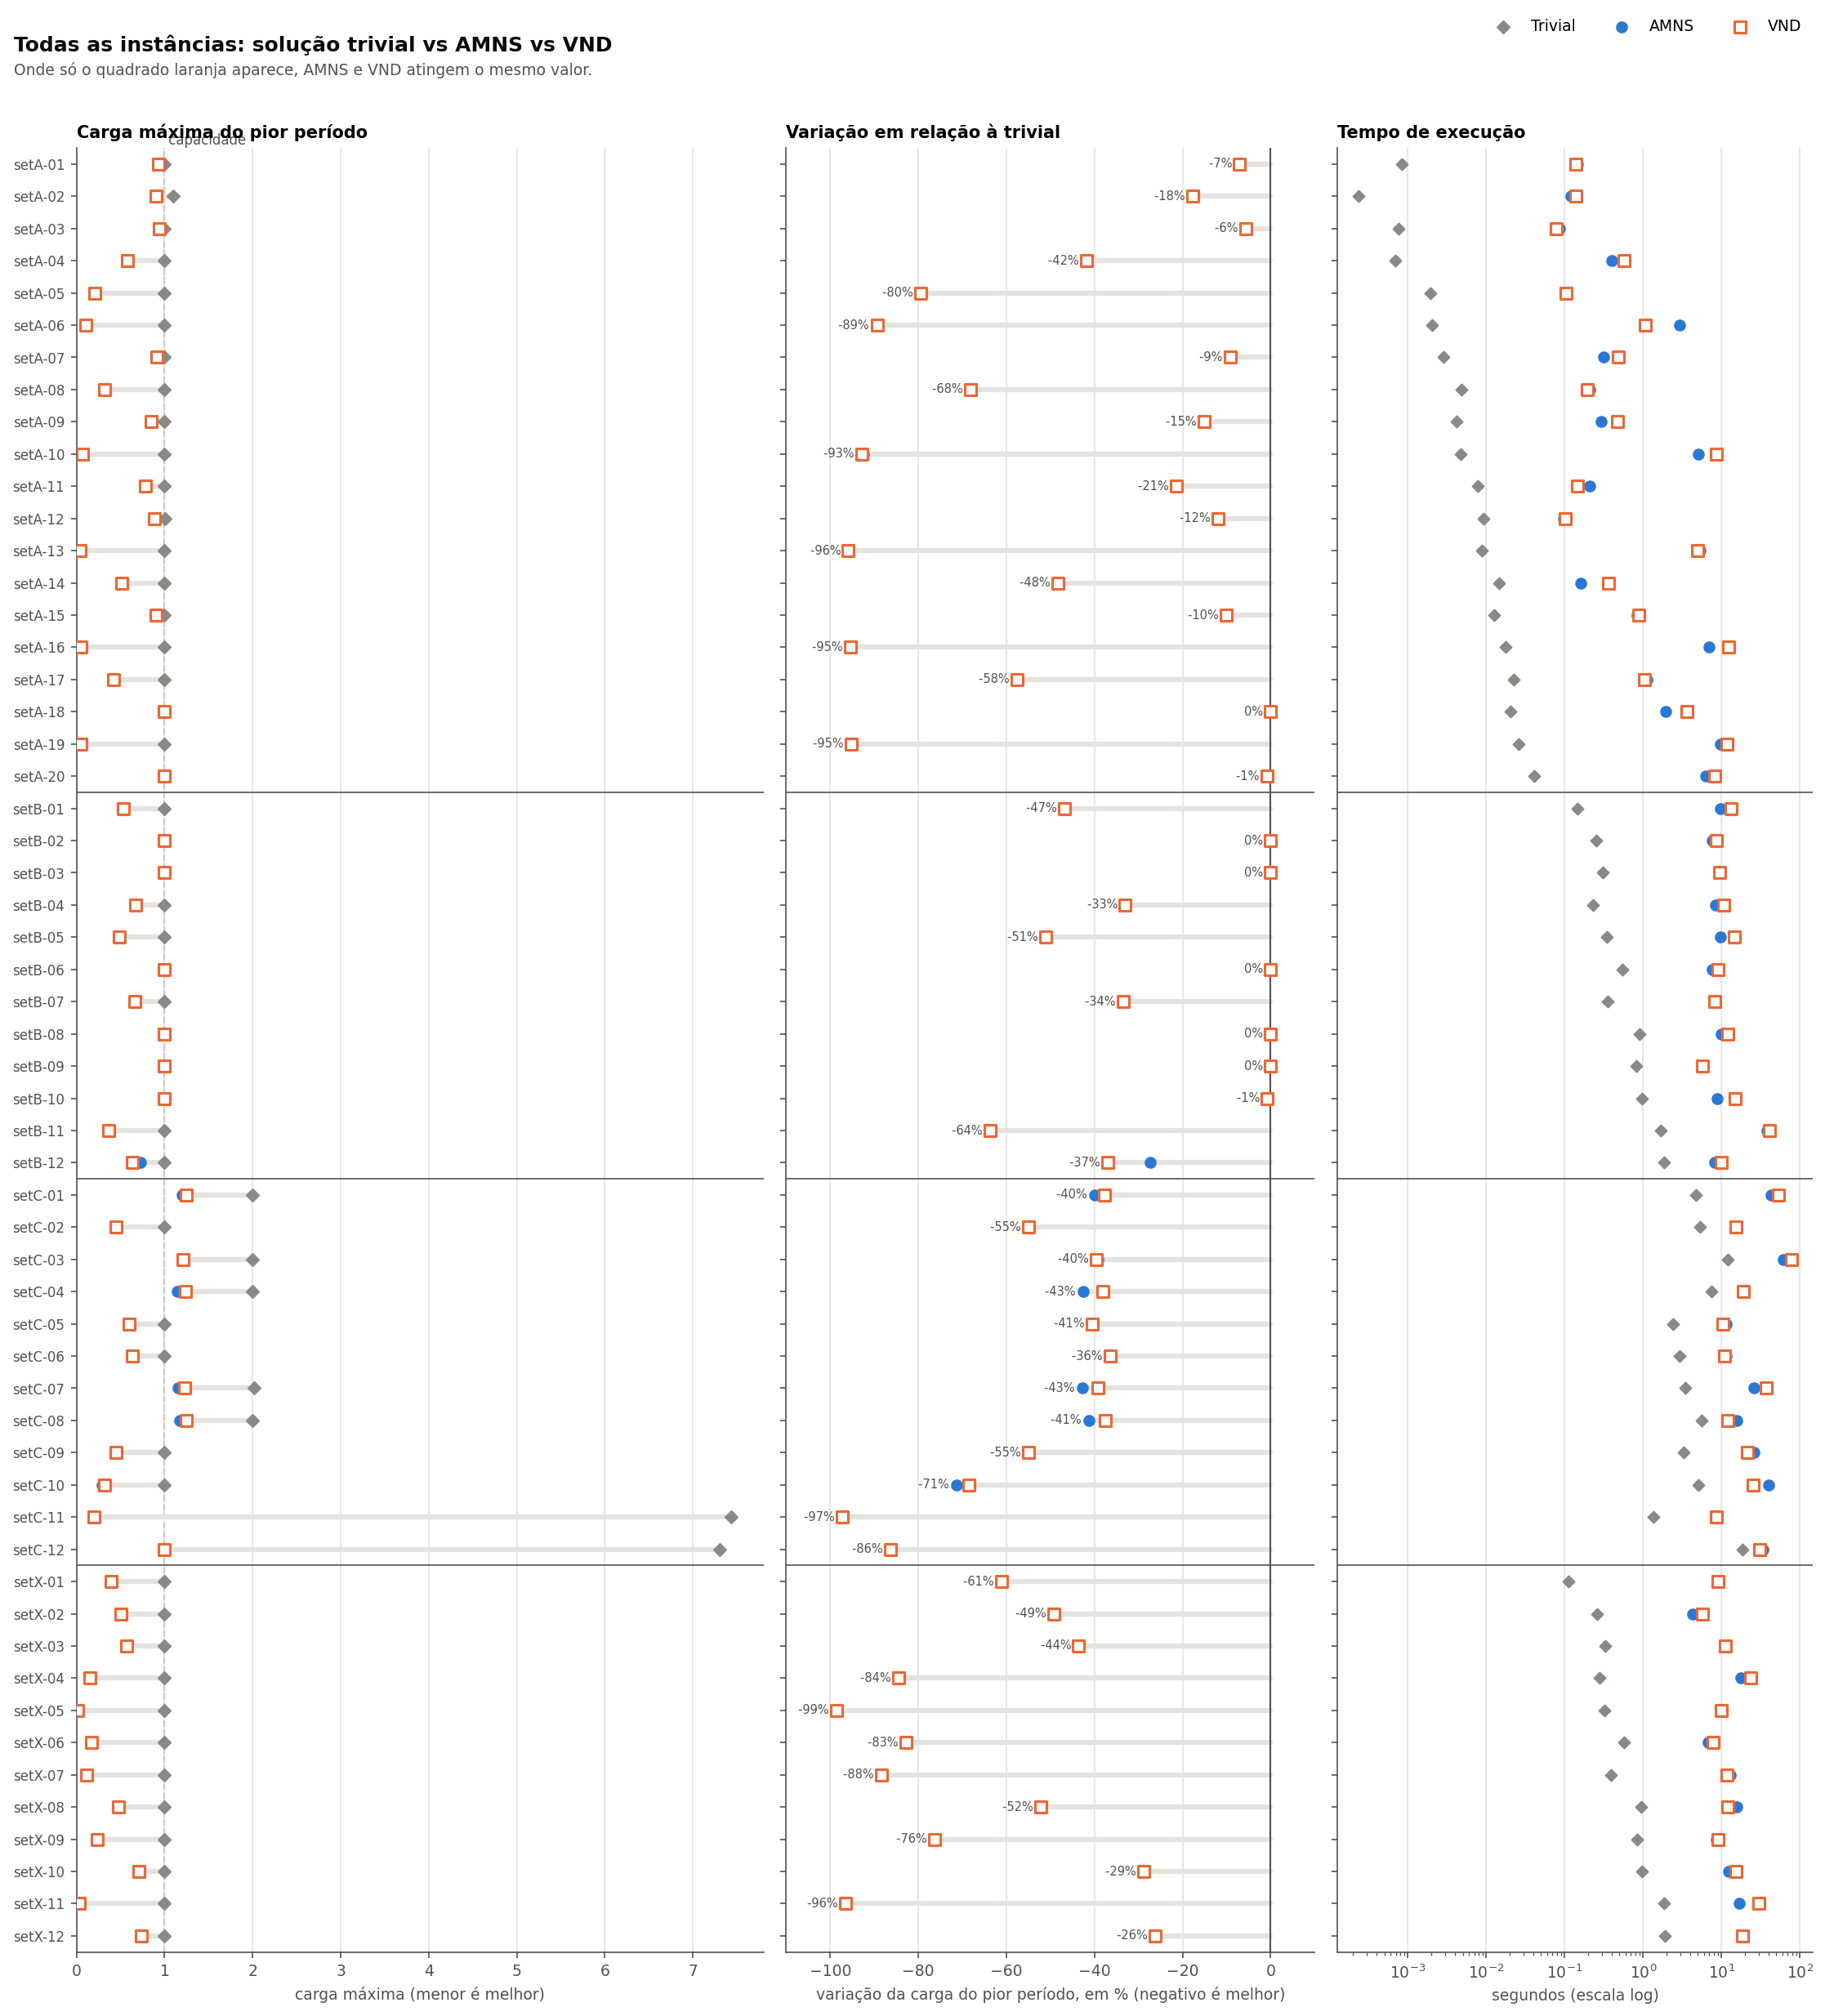
\includegraphics[width=\textwidth]{figuras/resumo_instancias.png}
\caption{MLU do pior período, variação em relação à solução trivial e tempo de execução, por instância. Onde só o quadrado laranja aparece, AMNS e VND atingem o mesmo valor.}
\label{fig:resumo}
\end{figure}

\begin{figure}[H]
\centering
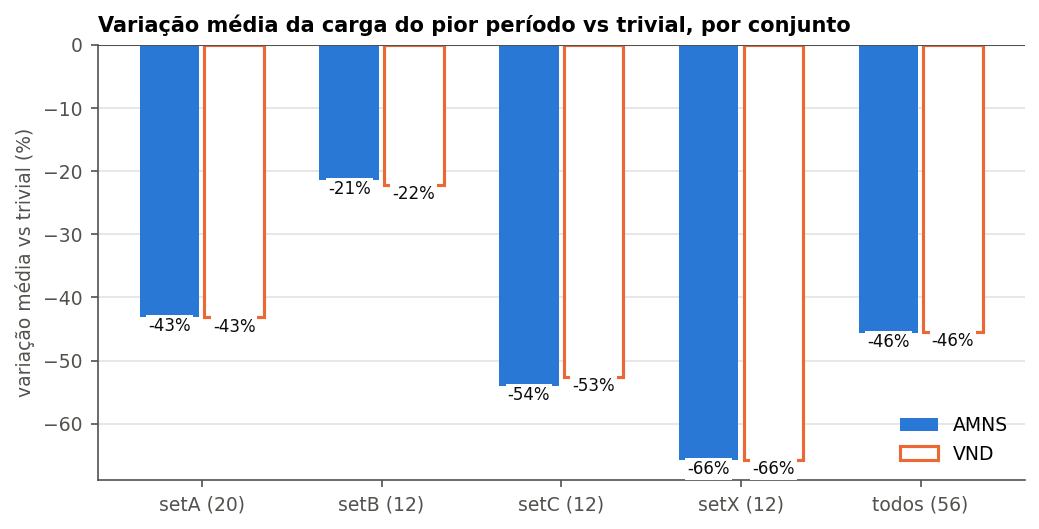
\includegraphics[width=0.75\textwidth]{figuras/resumo_conjuntos.png}
\caption{Variação média da MLU do pior período em relação à solução trivial, por conjunto de instâncias.}
\label{fig:porconjunto}
\end{figure}

\begin{table}[H]
\centering
\caption{MLU do pior período (avaliador oficial) e tempo de execução por instância.}
\label{tab:resultados}
\footnotesize
\begin{tabular}{lrrrrrrr}
\toprule
 & \multicolumn{3}{c}{MLU do pior período} & \multicolumn{2}{c}{Variação vs. trivial} & \multicolumn{2}{c}{Tempo (s)} \\
\cmidrule(lr){2-4} \cmidrule(lr){5-6} \cmidrule(lr){7-8}
Instância & Trivial & AMNS & VND & AMNS & VND & AMNS & VND \\
\midrule
setA-01 & 1{,}000 & 0{,}929 & 0{,}929 & $-$7{,}1\% & $-$7{,}1\% & 0{,}1 & 0{,}1 \\
setA-02 & 1{,}098 & 0{,}903 & 0{,}903 & $-$17{,}8\% & $-$17{,}8\% & 0{,}1 & 0{,}1 \\
setA-03 & 1{,}000 & 0{,}944 & 0{,}944 & $-$5{,}7\% & $-$5{,}7\% & 0{,}1 & 0{,}1 \\
setA-04 & 1{,}000 & 0{,}582 & 0{,}582 & $-$41{,}8\% & $-$41{,}8\% & 0{,}4 & 0{,}6 \\
setA-05 & 1{,}000 & 0{,}205 & 0{,}205 & $-$79{,}5\% & $-$79{,}5\% & 0{,}1 & 0{,}1 \\
setA-06 & 1{,}000 & 0{,}106 & 0{,}107 & $-$89{,}4\% & $-$89{,}3\% & 2{,}9 & 1{,}1 \\
setA-07 & 1{,}000 & 0{,}908 & 0{,}908 & $-$9{,}2\% & $-$9{,}2\% & 0{,}3 & 0{,}5 \\
setA-08 & 1{,}000 & 0{,}319 & 0{,}319 & $-$68{,}1\% & $-$68{,}1\% & 0{,}2 & 0{,}2 \\
setA-09 & 1{,}000 & 0{,}850 & 0{,}850 & $-$15{,}0\% & $-$15{,}0\% & 0{,}3 & 0{,}5 \\
setA-10 & 1{,}000 & 0{,}076 & 0{,}072 & $-$92{,}4\% & $-$92{,}8\% & 5{,}0 & 8{,}6 \\
setA-11 & 1{,}000 & 0{,}786 & 0{,}786 & $-$21{,}4\% & $-$21{,}4\% & 0{,}2 & 0{,}1 \\
setA-12 & 1{,}000 & 0{,}880 & 0{,}880 & $-$12{,}0\% & $-$12{,}0\% & 0{,}1 & 0{,}1 \\
setA-13 & 1{,}000 & 0{,}041 & 0{,}041 & $-$95{,}9\% & $-$95{,}9\% & 5{,}4 & 5{,}0 \\
setA-14 & 1{,}000 & 0{,}518 & 0{,}518 & $-$48{,}2\% & $-$48{,}2\% & 0{,}2 & 0{,}4 \\
setA-15 & 1{,}000 & 0{,}899 & 0{,}899 & $-$10{,}1\% & $-$10{,}1\% & 0{,}8 & 0{,}9 \\
setA-16 & 1{,}000 & 0{,}047 & 0{,}045 & $-$95{,}3\% & $-$95{,}5\% & 7{,}0 & 12{,}4 \\
setA-17 & 1{,}000 & 0{,}424 & 0{,}424 & $-$57{,}6\% & $-$57{,}6\% & 1{,}1 & 1{,}1 \\
setA-18 & 1{,}000 & 1{,}000 & 1{,}000 & 0{,}0\% & 0{,}0\% & 2{,}0 & 3{,}6 \\
setA-19 & 1{,}000 & 0{,}047 & 0{,}047 & $-$95{,}3\% & $-$95{,}3\% & 9{,}7 & 11{,}9 \\
setA-20 & 1{,}000 & 0{,}991 & 0{,}991 & $-$0{,}9\% & $-$0{,}9\% & 6{,}4 & 8{,}2 \\
\midrule
setB-01 & 1{,}000 & 0{,}533 & 0{,}532 & $-$46{,}7\% & $-$46{,}8\% & 9{,}7 & 13{,}2 \\
setB-02 & 1{,}000 & 1{,}000 & 1{,}000 & 0{,}0\% & 0{,}0\% & 7{,}6 & 8{,}7 \\
setB-03 & 1{,}000 & 1{,}000 & 1{,}000 & 0{,}0\% & 0{,}0\% & 9{,}7 & 9{,}6 \\
setB-04 & 1{,}000 & 0{,}670 & 0{,}670 & $-$33{,}0\% & $-$33{,}0\% & 8{,}3 & 10{,}7 \\
setB-05 & 1{,}000 & 0{,}489 & 0{,}489 & $-$51{,}1\% & $-$51{,}1\% & 9{,}6 & 14{,}8 \\
setB-06 & 1{,}000 & 1{,}000 & 1{,}000 & 0{,}0\% & 0{,}0\% & 7{,}6 & 9{,}0 \\
setB-07 & 1{,}000 & 0{,}665 & 0{,}665 & $-$33{,}5\% & $-$33{,}5\% & 8{,}2 & 8{,}2 \\
setB-08 & 1{,}000 & 1{,}000 & 1{,}000 & 0{,}0\% & 0{,}0\% & 9{,}9 & 12{,}0 \\
setB-09 & 1{,}000 & 1{,}000 & 1{,}000 & 0{,}0\% & 0{,}0\% & 5{,}9 & 5{,}7 \\
setB-10 & 1{,}000 & 0{,}992 & 0{,}992 & $-$0{,}8\% & $-$0{,}8\% & 8{,}8 & 15{,}1 \\
setB-11 & 1{,}000 & 0{,}364 & 0{,}364 & $-$63{,}6\% & $-$63{,}6\% & 38{,}4 & 40{,}9 \\
setB-12 & 1{,}000 & 0{,}726 & 0{,}630 & $-$27{,}4\% & $-$37{,}0\% & 8{,}2 & 9{,}8 \\
\midrule
setC-01 & 2{,}000 & 1{,}200 & 1{,}244 & $-$40{,}0\% & $-$37{,}8\% & 42{,}5 & 53{,}5 \\
setC-02 & 1{,}000 & 0{,}450 & 0{,}450 & $-$55{,}0\% & $-$55{,}0\% & 14{,}9 & 15{,}3 \\
setC-03 & 2{,}000 & 1{,}215 & 1{,}207 & $-$39{,}2\% & $-$39{,}6\% & 61{,}5 & 77{,}7 \\
setC-04 & 2{,}000 & 1{,}149 & 1{,}237 & $-$42{,}6\% & $-$38{,}1\% & 18{,}8 & 18{,}9 \\
setC-05 & 1{,}000 & 0{,}594 & 0{,}594 & $-$40{,}5\% & $-$40{,}5\% & 11{,}4 & 10{,}4 \\
setC-06 & 1{,}000 & 0{,}635 & 0{,}635 & $-$36{,}5\% & $-$36{,}5\% & 11{,}6 & 11{,}0 \\
setC-07 & 2{,}015 & 1{,}153 & 1{,}225 & $-$42{,}8\% & $-$39{,}2\% & 26{,}1 & 36{,}9 \\
setC-08 & 2{,}000 & 1{,}174 & 1{,}248 & $-$41{,}3\% & $-$37{,}6\% & 15{,}8 & 12{,}2 \\
setC-09 & 1{,}000 & 0{,}450 & 0{,}450 & $-$55{,}0\% & $-$55{,}0\% & 26{,}2 & 21{,}2 \\
setC-10 & 1{,}000 & 0{,}286 & 0{,}315 & $-$71{,}4\% & $-$68{,}5\% & 40{,}3 & 25{,}4 \\
setC-11 & 7{,}433 & 0{,}200 & 0{,}200 & $-$97{,}3\% & $-$97{,}3\% & 8{,}5 & 8{,}6 \\
setC-12 & 7{,}307 & 1{,}000 & 1{,}000 & $-$86{,}3\% & $-$86{,}3\% & 33{,}7 & 30{,}8 \\
\midrule
setX-01 & 1{,}000 & 0{,}388 & 0{,}388 & $-$61{,}2\% & $-$61{,}2\% & 9{,}2 & 9{,}1 \\
setX-02 & 1{,}000 & 0{,}508 & 0{,}508 & $-$49{,}2\% & $-$49{,}2\% & 4{,}3 & 5{,}7 \\
setX-03 & 1{,}000 & 0{,}564 & 0{,}564 & $-$43{,}6\% & $-$43{,}6\% & 11{,}0 & 11{,}2 \\
setX-04 & 1{,}000 & 0{,}155 & 0{,}155 & $-$84{,}5\% & $-$84{,}5\% & 17{,}6 & 23{,}6 \\
setX-05 & 1{,}000 & 0{,}014 & 0{,}014 & $-$98{,}6\% & $-$98{,}6\% & 9{,}8 & 9{,}9 \\
setX-06 & 1{,}000 & 0{,}172 & 0{,}172 & $-$82{,}8\% & $-$82{,}8\% & 6{,}8 & 7{,}7 \\
setX-07 & 1{,}000 & 0{,}117 & 0{,}117 & $-$88{,}3\% & $-$88{,}3\% & 13{,}1 & 11{,}8 \\
setX-08 & 1{,}000 & 0{,}479 & 0{,}479 & $-$52{,}1\% & $-$52{,}1\% & 15{,}8 & 11{,}9 \\
setX-09 & 1{,}000 & 0{,}238 & 0{,}238 & $-$76{,}2\% & $-$76{,}2\% & 8{,}5 & 9{,}1 \\
setX-10 & 1{,}000 & 0{,}711 & 0{,}711 & $-$28{,}9\% & $-$28{,}9\% & 12{,}4 & 15{,}3 \\
setX-11 & 1{,}000 & 0{,}035 & 0{,}035 & $-$96{,}5\% & $-$96{,}5\% & 17{,}0 & 30{,}2 \\
setX-12 & 1{,}000 & 0{,}737 & 0{,}737 & $-$26{,}3\% & $-$26{,}3\% & 18{,}0 & 18{,}7 \\
\bottomrule
\end{tabular}
\end{table}


\section{\uppercase{Comparação entre AMNS e VND}}

AMNS e VND atingem a mesma MLU do pior período em 43 das 56 instâncias; a AMNS é melhor em 7 (cinco delas no conjunto C) e a VND em 6. A semelhança se explica pela fase robusta, compartilhada pelos dois métodos: como os orçamentos impedem mudanças relevantes depois do período 0, o resultado final é determinado em grande parte pelo planejamento do período 0 feito por essa fase.

O tempo total é de 629 segundos para a AMNS e 699 segundos para a VND; nos conjuntos A, B e X, sem o conjunto C, são 318 e 377 segundos. Em uma versão anterior, a AMNS só parava após 400 chamadas de vizinhança sem nova melhor solução, e qualquer melhora nos critérios de desempate reiniciava essa contagem; nos períodos após o primeiro, em que quase nada pode ser melhorado, ela gastava em média 749 chamadas por período contra 89 da VND, e o tempo total nos conjuntos A, B e X era de 557 segundos. Com a parada após 100 chamadas sem progresso na carga máxima, esse tempo caiu para cerca de 210 segundos, com o mesmo resultado em 40 das 44 instâncias.

A Figura~\ref{fig:overview} detalha a instância setA-02. A solução trivial ultrapassa a capacidade no período 1, após uma intervenção, enquanto AMNS e VND mantêm os dois períodos abaixo de 1. O painel dos 30 enlaces mais carregados mostra o efeito da otimização: as cargas dos enlaces mais carregados caem, ao custo de um pequeno aumento da carga média, porque os desvios alongam as rotas.

\begin{figure}[H]
\centering
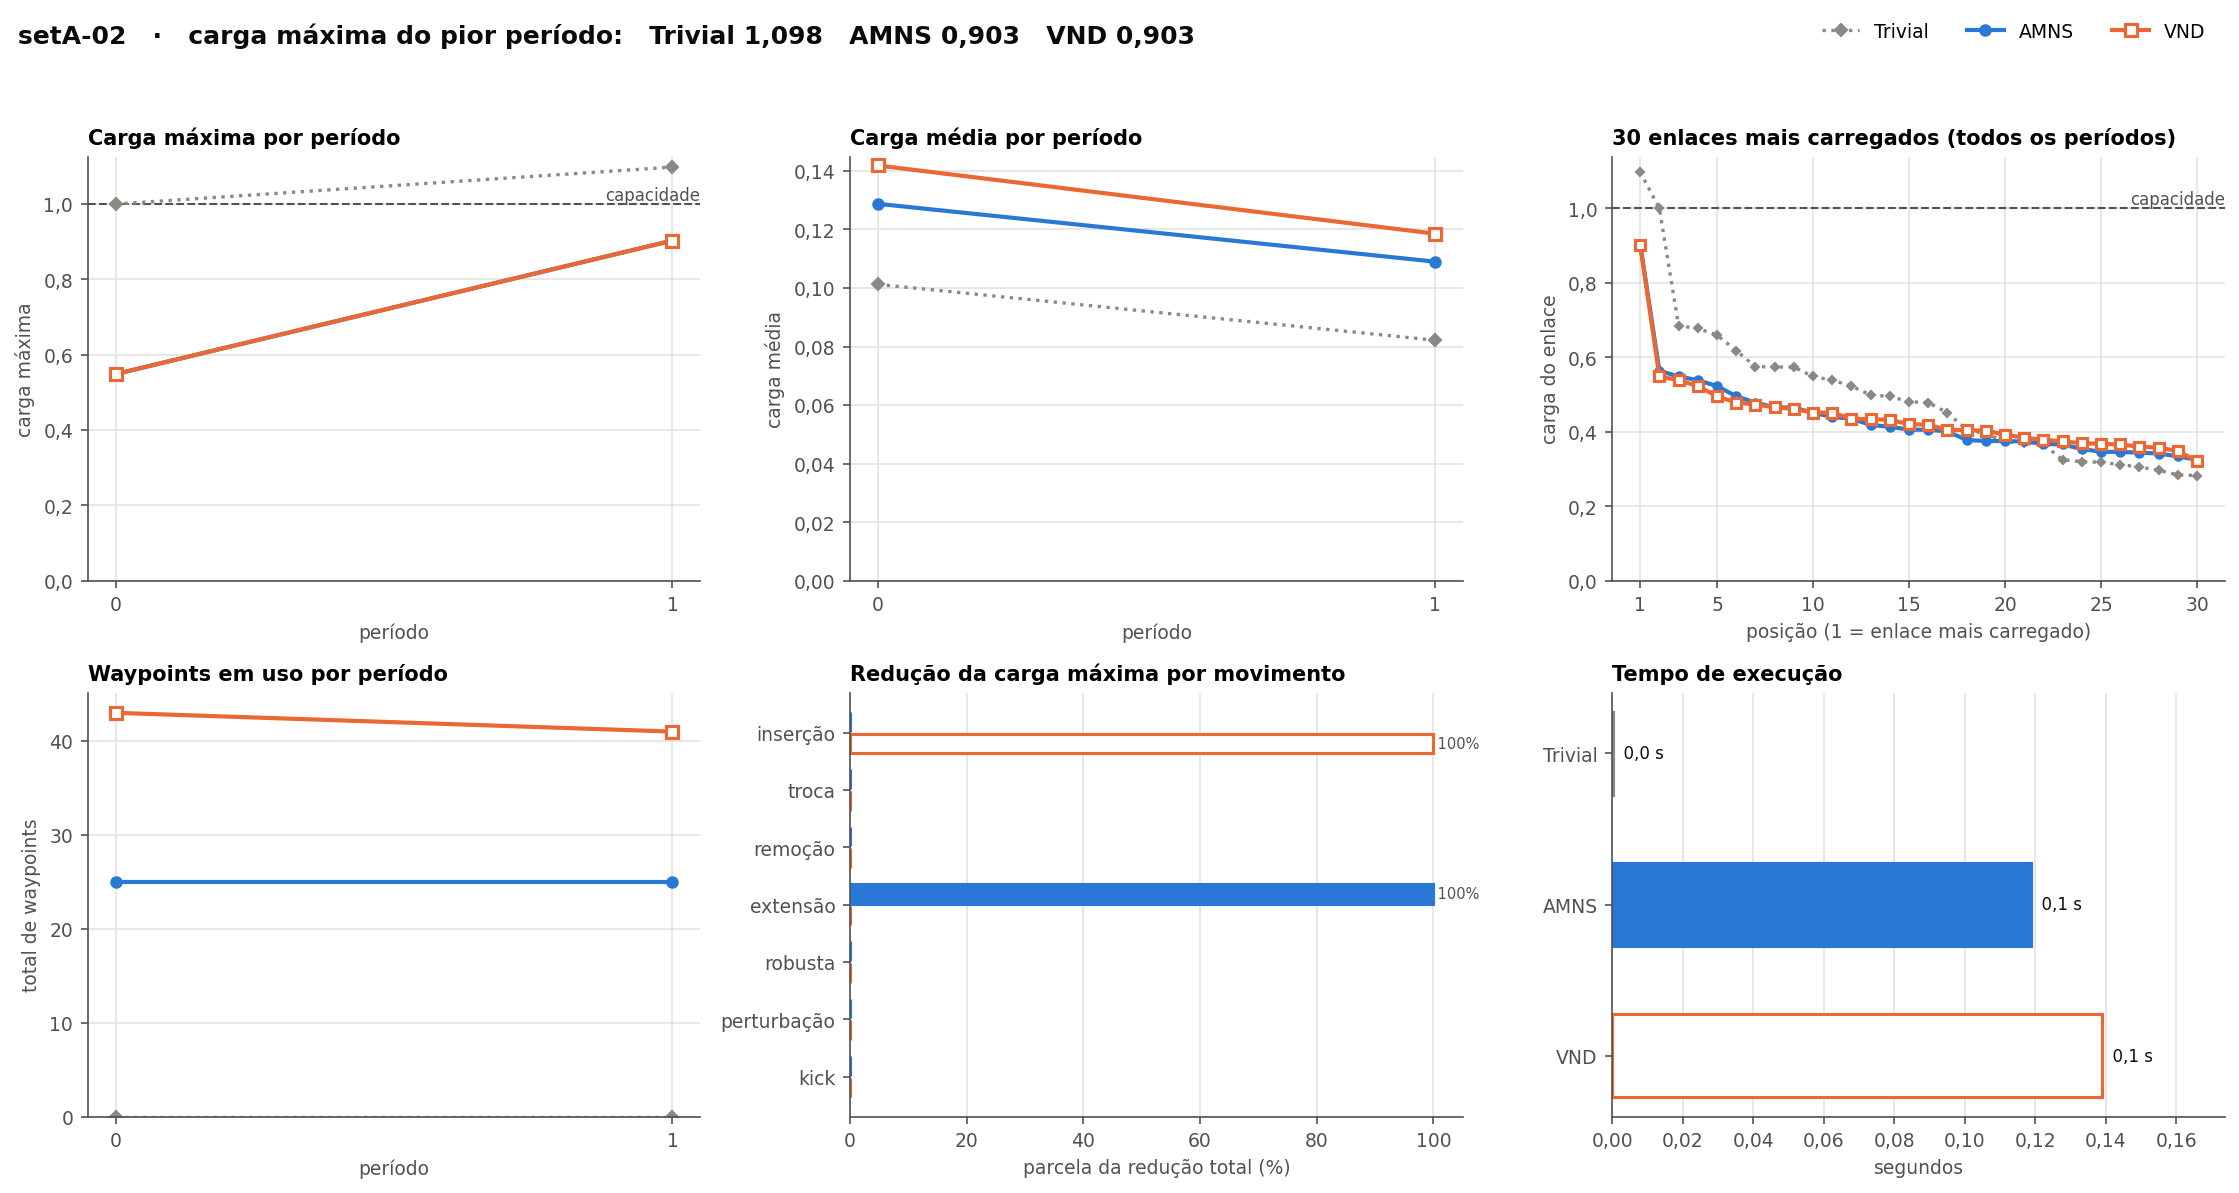
\includegraphics[width=\textwidth]{figuras/setA-02_visao_geral.png}
\caption{Instância setA-02: MLU e carga média por período, 30 enlaces mais carregados, \textit{waypoints} em uso, redução da MLU por movimento e tempo de execução.}
\label{fig:overview}
\end{figure}

A Figura~\ref{fig:historico} mostra a evolução da busca na instância setB-05. A maior parte da redução ocorre no período 0, nas primeiras iterações; nos períodos seguintes, o orçamento permite apenas pequenos ajustes, e só o período 9 apresenta melhora.

\begin{figure}[H]
\centering
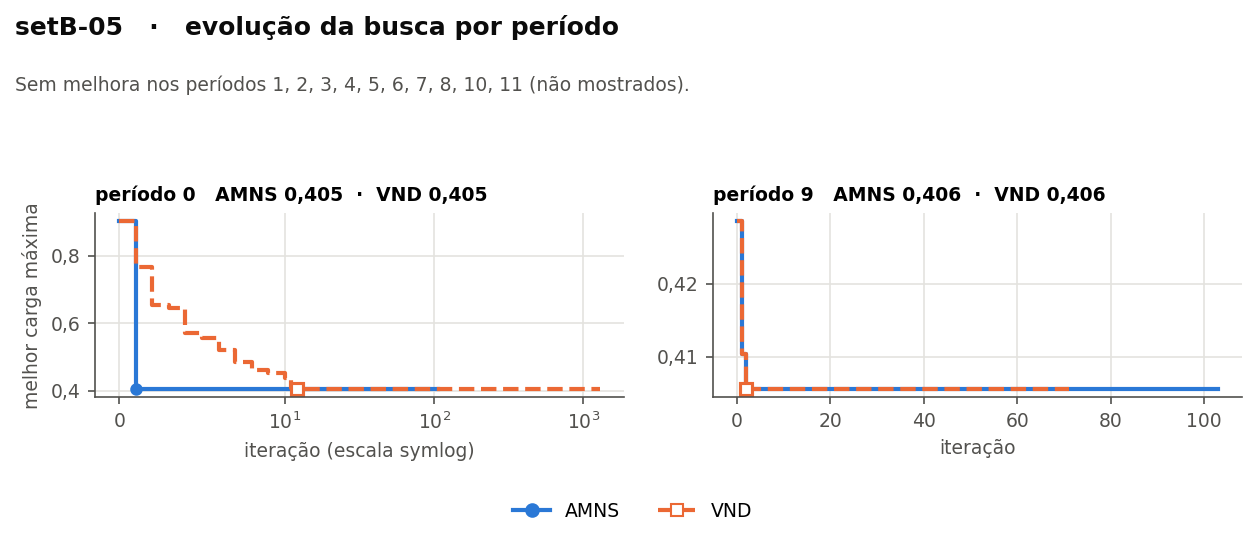
\includegraphics[width=\textwidth]{figuras/setB-05_historico.png}
\caption{Instância setB-05: evolução da melhor MLU ao longo da busca, nos períodos em que houve melhora.}
\label{fig:historico}
\end{figure}

\section{\uppercase{Inserção Dupla de \textit{Waypoints}}}
\label{sec:insercao_dupla}

Foi testado um movimento adicional, a inserção dupla, que insere dois \textit{waypoints} de uma vez em um segmento que atravessa o corte crítico. A motivação é o caso em que um único \textit{waypoint} não resolve: todos os caminhos mínimos até o nó de desvio útil passam pelo próprio enlace congestionado, e só um par $(x, y)$ consegue alcançar $y$ pelo outro lado. Os primeiros \textit{waypoints} $y$ candidatos são os vizinhos dos extremos de cada enlace crítico (outros vizinhos de entrada do nó de chegada e outros vizinhos de saída do nó de partida) e os 6 melhores nós de desvio pela carga residual; para cada $y$, os parceiros $x$ são os 6 melhores nós de desvio antes ou depois de $y$. Na AMNS o movimento recebeu peso inicial 1; na VND foi colocado logo após a inserção simples.

As 56 instâncias foram resolvidas com e sem o movimento, nas mesmas condições. A Tabela~\ref{tab:insercao_dupla} resume o resultado, considerando iguais as diferenças de MLU menores que 0,5\%.

\begin{table}[H]
\centering
\caption{Efeito da inserção dupla: instâncias em que a MLU do pior período melhora ou piora mais de 0,5\%, variação média e tempo total.}
\label{tab:insercao_dupla}
\begin{tabular}{lrrrrr}
\toprule
Método & Melhora & Piora & Variação média & Tempo sem (s) & Tempo com (s) \\
\midrule
AMNS & 4 & 5 & $-$0{,}06\% & 629 & 1987 \\
VND & 0 & 5 & $+$0{,}65\% & 699 & 2343 \\
\bottomrule
\end{tabular}
\end{table}

O movimento não compensa. Na AMNS, os ganhos (setB-12 $-$11,3\%, setC-10 $-$10,7\%, setC-01 $-$5,0\%, setC-03 $-$3,7\%) são anulados pelas perdas (setA-16 $+$13,0\%, setA-06 $+$6,7\%, setC-07 $+$5,2\%), e na VND só há perdas. O tempo total aumenta cerca de 3,2 vezes na AMNS e 3,4 vezes na VND, porque cada chamada avalia dezenas de pares: nos períodos após o primeiro, a inserção dupla consumiu cerca de 1400 segundos na AMNS e 1600 na VND, com menos de 1\% de chamadas bem-sucedidas, enquanto a inserção simples consumiu cerca de 25 segundos. No período 0 ela melhora a solução em 17\% das chamadas na AMNS, mas a inserção simples já faz a maior parte do trabalho, e a fase robusta já usa desvios com dois \textit{waypoints}. As perdas vêm do tempo tirado das outras vizinhanças: com o mesmo limite de tempo por período, sobram menos iterações para a inserção simples e a perturbação. Por isso, a inserção dupla ficou desativada na versão final dos métodos, e todos os demais resultados deste capítulo foram obtidos sem ela.

\section{\uppercase{Tamanho das Listas de Candidatos}}
\label{sec:listas_candidatos}

Os tamanhos das listas de candidatos (16 nós por posição, 32 no período 0, 64 para as demandas no pico da fase robusta e 48 demandas por chamada da extensão e da fase robusta) são fixos, independentemente do tamanho da instância. Foi testada uma regra que os torna proporcionais à instância: cada lista de nós passa a ser uma fração do número de nós $N$ (4\% de $N$ para a lista principal, 8\% no período 0, 16\% para as demandas no pico da fase robusta), e a janela de demandas passa a ser 1\% do número de demandas, com limites inferior e superior. Para $N = 400$, o maior tamanho de rede do conjunto A, a regra reproduz os tamanhos fixos.

Foram avaliadas duas versões nas 56 instâncias. Na primeira, as listas crescem até 3 vezes os tamanhos fixos nas redes grandes. A qualidade praticamente não mudou (variação média da MLU do pior período de $+$0,37\% na AMNS e $-$0,08\% na VND), mas o tempo total aumentou cerca de 47\% (de 629 para 926 segundos na AMNS e de 699 para 942 na VND), quase todo no conjunto C, cujas redes de 800 a 3900 nós atingem os limites superiores. Como o tempo por período é fixo, listas mais longas significam menos iterações, e as duas coisas se compensam. Na segunda versão, os limites superiores são os tamanhos fixos, de modo que as listas só diminuem nas redes pequenas. Nos conjuntos B, C e X, cujas redes são em geral maiores, as listas ficam quase sempre nos tamanhos fixos e o resultado é praticamente o da versão fixa; no conjunto A o efeito é misto: setA-10 e setA-16 melhoram de 4\% a 6\%, mas setA-02, com 30 nós, piora 21,6\% na AMNS, nas duas versões. Como as instâncias pequenas são resolvidas em menos de um segundo, reduzir suas listas não economiza tempo útil.

Esses experimentos também mostram a variabilidade de execuções únicas com limite de tempo: em setC-10, cujos tamanhos de lista são idênticos nas versões fixa e limitada, a MLU variou cerca de 16\% entre as execuções, com os dois métodos. Diferenças desse porte em instâncias isoladas não são, portanto, significativas. Como nenhuma das versões melhorou o resultado médio, os tamanhos fixos foram mantidos.

\section{\uppercase{Discussão}}

Os resultados mostram que o \textit{Segment Routing} reduz substancialmente a carga máxima mesmo com poucos \textit{waypoints} por demanda e com orçamentos de reconfiguração muito restritos. Três observações orientam a continuidade do trabalho:

\begin{itemize}
    \item \textbf{O período 0 decide o resultado.} Com orçamentos pequenos, as rotas do período 0 valem para todo o horizonte. Planejá-las considerando as intervenções futuras foi o fator que mais contribuiu para os resultados.
    \item \textbf{Decisões míopes nos períodos seguintes.} Nos períodos após o primeiro, cada movimento é avaliado apenas pela carga do próprio período, mas suas mudanças permanecem nos períodos seguintes. Na instância setB-12, mudanças feitas nos períodos 2 e 3 elevaram a MLU dos períodos 4 a 7 de 0,630 para 0,726 em uma das execuções da AMNS.
    \item \textbf{AMNS e VND são equivalentes neste contexto.} Como a fase robusta domina o resultado, a escolha entre as duas estratégias de busca afeta mais o tempo de execução do que a qualidade final.
\end{itemize}

\chapter{CONCLUSÕES E TRABALHOS FUTUROS}
\label{cap:conclusao}

\section{\uppercase{Conclusões}}

Este trabalho tratou o problema de \textit{Segment Routing} adaptativo no tempo (T-ASR), proposto no desafio EURO/ROADEF 2026. Foram desenvolvidas duas meta-heurísticas de busca em vizinhança, AMNS e VND com perturbação, que compartilham a avaliação das cargas, a função objetivo, as vizinhanças e uma fase robusta para o primeiro período.

A avaliação das cargas reproduz exatamente o avaliador oficial, incluindo a divisão de tráfego por ECMP, o que garante que a busca otimiza o mesmo critério usado na avaliação. A principal contribuição metodológica é a fase robusta: como os orçamentos de reconfiguração são pequenos, as rotas do primeiro período valem para todo o horizonte, e escolhê-las considerando as intervenções de todos os períodos foi decisivo. Para avaliar esses cenários de forma eficiente, apenas os segmentos afetados por cada intervenção são recalculados, com distâncias reparadas a partir das do primeiro período.

Nas 56 instâncias dos conjuntos A, B, C e X, os dois métodos reduziram a utilização máxima do pior período em cerca de 46\% em média em relação ao roteamento IGP sem otimização e produziram soluções válidas segundo o avaliador oficial. Nos conjuntos A, B e X, eliminaram todas as violações de capacidade; no conjunto C, reduziram cargas de até 7,4 vezes a capacidade, mas em cinco instâncias a utilização máxima continua entre 1,15 e 1,25. AMNS e VND alcançaram resultados equivalentes, com tempos totais de 629 e 699 segundos. Um movimento adicional de inserção dupla de \textit{waypoints} foi testado e descartado: não melhorou a qualidade média e triplicou o tempo de execução.

\section{\uppercase{Trabalhos Futuros}}

\begin{itemize}
    \item \textbf{Sobrecargas do conjunto C}: verificar se as cargas acima de 1 que restam em cinco instâncias do conjunto C são inevitáveis (por exemplo, por um limite inferior calculado sobre os enlaces que nenhum desvio evita) ou se podem ser eliminadas.
    \item \textbf{Decisões não míopes nos períodos seguintes}: avaliar os movimentos dos períodos após o primeiro também nos períodos que vêm depois, estendendo a fase robusta, para evitar que mudanças locais elevem a carga mais adiante.
    \item \textbf{Estudo de ablação das vizinhanças}: medir a contribuição de cada movimento (inserção, troca, remoção, extensão, perturbação e os movimentos da fase robusta) desativando-os um a um, para simplificar os métodos e redistribuir o tempo de busca.
    \item \textbf{Objetivo lexicográfico completo}: comparar as soluções pelo vetor ordenado de cargas de todos os períodos, como no critério oficial, e não apenas pela aproximação usada na busca.
    \item \textbf{Múltiplas execuções}: repetir os experimentos com sementes diferentes para medir a variabilidade dos métodos.
\end{itemize}



%------------------------------------------------------------------------------

% Bibliografia desativada por enquanto (ainda sem citacoes no texto).
%\renewcommand{\bibname}{REFERÊNCIAS}
%\label{bib:begin}
%\renewcommand\bibname{\centerline{REFERÊNCIAS}\global\def\bibname{REFERÊNCIAS}}
%
%\bibliographystyle{bibformat}
%\bibliography{referencias}
%\label{bib:end}

%\appendix
%\input{./capitulos/appendix.tex}


\end{document}
